\chapter{Triaxial}
\label{sec:Triaxial}
\section{Triaxial Potentials}


\subsection{Logarithmic Triaxial Density Profile}\label{sec:LM10}

Motivated by the fact that the models of the Milky Way Dark Matter halo
at that time can not reproduce the Sgr stream. Mainly because in axisietric
potentials it is not possible to fit the angular precession and the the
distance of the stream. \cite{Law09} propose a triaxial halo Eq.\ref{eq:LMpotential}
which is also in agreement with the CDM paradigm that predicts triaxial halos
rather than  spherical \cite{Lee03}. \cite{Law09} report results of the orbital
integration in which they find that the best fit in their triaxial halo is for $q_z = 1.25$,
 $q_1 = 1.5$ and $\phi=90$. \cite{Law10} made N-body simulations in which they
include the triaxial halo potential.

\begin{equation}\label{eq:LMpotential}
\Phi = v^2_{halo} ln(C_1 x^2 + C_2y^2 + C_3 xy + (z/q_z)^2+ r_{halo}^2)
\end{equation}

Where the constants $C_1, C_2, C_3$ are defined as:
%$R, r$ (Cylindrical, spherical)

\begin{equation}
C_1 = \left( \dfrac{cos^2 \phi}{q_1^2} + \dfrac{sin^2 \phi}{q_2^2}   \right)
\end{equation}

\begin{equation}
C_2 = \left( \dfrac{cos^2 \phi}{q_2^2} + \dfrac{sin^2 \phi}{q_1^2} \right)
\end{equation}

\begin{equation}
C_3 = 2 sin \phi cos\phi \left( \dfrac{1}{q_1^2} - \dfrac{1}{q_2^2} \right)
\end{equation}

\begin{figure}\label{fig:Logarithmic}
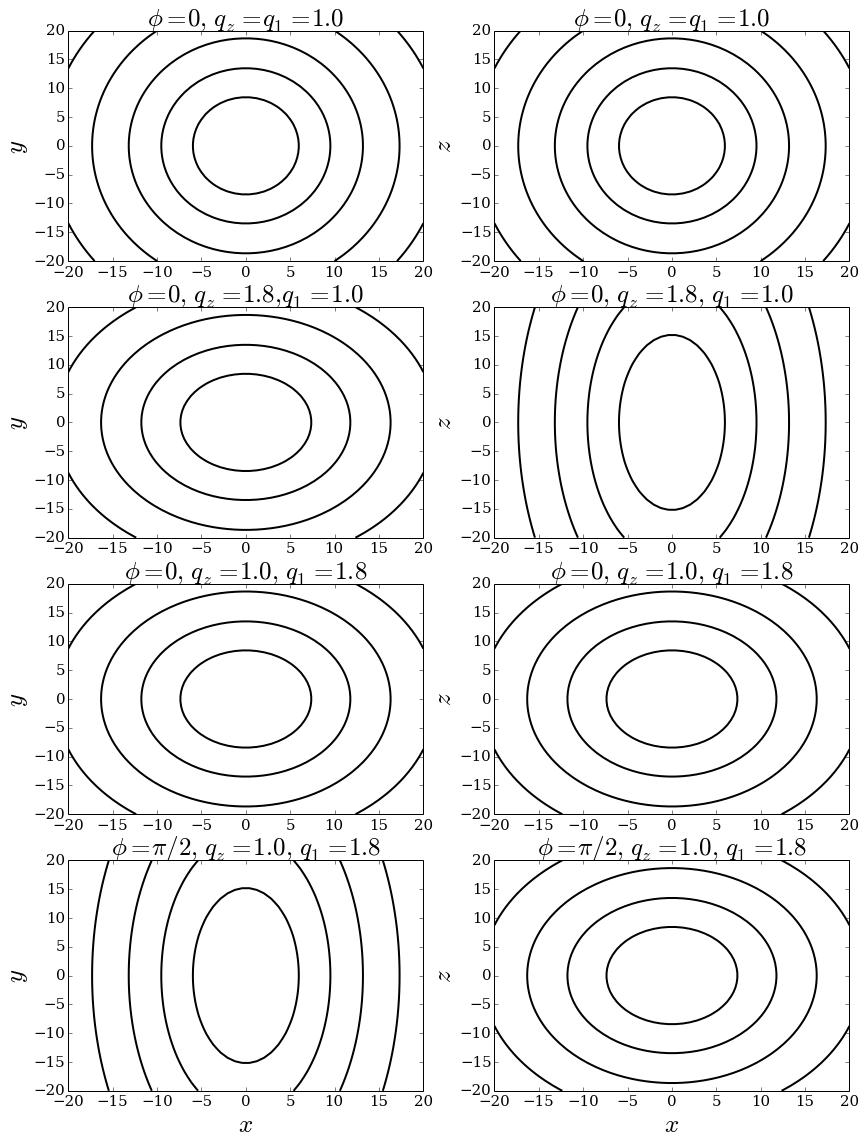
\includegraphics[scale=0.5]{../figures/triaxial_potential.png}
\caption{Logarithmic Triaxial Potential. In the top panel}
\end{figure}



From Eq.\ref{eq:LMpotential} we can derive the circular velocity $v_c$.

\begin{equation}
v_c^2 = r \nabla  \Phi 
\end{equation}

\begin{equation}
\nabla \Phi = \dfrac{d}{dx} \Phi \hat{i} + \dfrac{d}{dy} \Phi \hat{j} + \dfrac{d}{dz} \Phi \hat{k}
\end{equation}

\begin{equation}
\nabla \phi = v_{halo}^2  \left( \dfrac{(2C_1x + C_3 y)\hat{i} + (2C_2y + C_3x)\hat{j} + (2z/q_z^2)\hat{k}}{(C_1 x^2 + C_2 y^2 + C_3 x y + (z/q_z)^2 + r_{halo}^2)}    \right)
\end{equation}

\begin{equation}
v_c = v_{halo} \sqrt{ \dfrac{r((2C_1x + C_3 y)^2 + (2C_2y + C_3x)^2 + (2z/q_z^2)^2)^{1/2}}{(C_1 x^2 + C_2 y^2 + C_3 x y + (z/q_z)^2 + r_{halo}^2)} }
\end{equation}

\citep{LM10} fixed the value of $v_{halo}$ in order that the MW rotation curve reproduce the obervsed value of $v_{LSR}= 220 km/s$ at $R_{\odot}$
this implies that $v_{halo} = 135 km/s$. The rotation curve of is presented in Fig.\ref{vcLM10}, the MW rotation curve is also presented in
Fig.\ref{MWML10} all the paremeters of this rotation curve are summarized in Table\ref{tab:models}.

\begin{figure}[H]\label{fig:vcLM10}
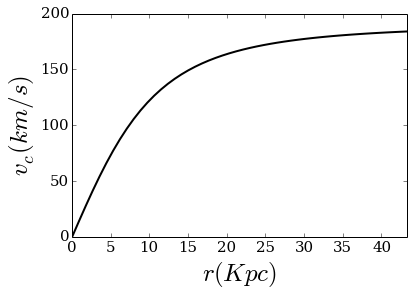
\includegraphics[scale=0.7]{../figures/vcLM10.png}
\end{figure}

